%% LyX 2.2.3 created this file.  For more info, see http://www.lyx.org/.
%% Do not edit unless you really know what you are doing.
\documentclass[oneside,reqno]{amsart}
\usepackage[T1]{fontenc}
\usepackage[utf8]{inputenc}
\pagestyle{plain}
\usepackage{amstext}
\usepackage{amsthm}
\usepackage{amssymb}
\usepackage{graphicx}
\usepackage{esint}
\usepackage[numbers]{natbib}
\usepackage[unicode=true,pdfusetitle,
 bookmarks=true,bookmarksnumbered=false,bookmarksopen=false,
 breaklinks=false,pdfborder={0 0 1},backref=section,colorlinks=false]
 {hyperref}

\makeatletter

%%%%%%%%%%%%%%%%%%%%%%%%%%%%%% LyX specific LaTeX commands.
%% Because html converters don't know tabularnewline
\providecommand{\tabularnewline}{\\}

%%%%%%%%%%%%%%%%%%%%%%%%%%%%%% Textclass specific LaTeX commands.
\numberwithin{equation}{section}
\numberwithin{figure}{section}

%%%%%%%%%%%%%%%%%%%%%%%%%%%%%% User specified LaTeX commands.
%2multibyte Version: 5.50.0.2960 CodePage: 1250
%\usepackage[notcite]{showkeys}
%\usepackage{graphicx}
%\usepackage{amscd}
%\usepackage{a4}
%unnumbered theorem environments
%\iffalse
%\usepackage[notcite]{showkeys}
%\usepackage{babel}
%\usepackage{babel}

\usepackage{amsthm}
\usepackage{mathrsfs}
%\usepackage[notcite]{showkeys}
\usepackage{amsthm}
\usepackage{datetime}
\usepackage{mathrsfs}
\usepackage{amsthm}
\usepackage{amsfonts}
\usepackage{comment}
\usepackage{graphicx}\setcounter{MaxMatrixCols}{30}
%TCIDATA{OutputFilter=latex2.dll}
%TCIDATA{Version=5.50.0.2960}
%TCIDATA{Codepage=1250}
%TCIDATA{CSTFile=amsart.cst}
%TCIDATA{Created=Wednesday, August 10, 2011 10:30:47}
%TCIDATA{LastRevised=Tuesday, November 03, 2015 14:08:24}
%TCIDATA{<META NAME="GraphicsSave" CONTENT="32">}
%TCIDATA{<META NAME="SaveForMode" CONTENT="1">}
%TCIDATA{BibliographyScheme=BibTeX}
%TCIDATA{<META NAME="DocumentShell" CONTENT="Articles\SW\bruce_plain">}
%TCIDATA{Language=American English}
%BeginMSIPreambleData
\providecommand{\U}[1]{\protect\rule{.1in}{.1in}}
%EndMSIPreambleData


\numberwithin{equation}{section}
\numberwithin{figure}{section}
\numberwithin{equation}{section}
\numberwithin{figure}{section}
\numberwithin{equation}{section}
\numberwithin{figure}{section}
\iffalse
\oddsidemargin= -0.2in
\evensidemargin= -0.2in
\textheight= 9in
\topmargin= -0.2in
\textwidth= 6.9in
\fi
\theoremstyle{plain}
\newtheorem{theorem}{Theorem}[section]
\newtheorem{corollary}[theorem]{Corollary}\newtheorem{lemma}[theorem]{Lemma}\newtheorem{convention}[theorem]{Convention}\newtheorem{mtheorem}[theorem]{Meta-Theorem}\newtheorem{proposition}[theorem]{Proposition}\newtheorem{htheorem}[theorem]{Heuristic Theorem}\newtheorem{axiom}{Axiom}\newtheorem{solution}[theorem]{Solution}\newtheorem{summary}[theorem]{Summary}\renewenvironment{proof}[1][Proof]{\textbf{#1.} }{\ \rule{0.5em}{0.5em}}
\theoremstyle{definition}
\newtheorem{definition}[theorem]{Definition}\newtheorem{comments}[theorem]{Comments}\newtheorem{notation}[theorem]{Notation}\newtheorem{notations}[theorem]{Notations}\newtheorem{example}[theorem]{Example}\theoremstyle{remark}
\newtheorem{remark}[theorem]{Remark}\newtheorem{remarks}[theorem]{Remarks}\newtheorem{fact}[theorem]{Fact}\theoremstyle{plain}
\newtheorem{conjecture}[]{Conjecture}\newtheorem{claim}[]{Claim}\newtheorem{computation}[]{Computation}\theoremstyle{definition}
\newtheorem{assumption}[]{Assumption}\newtheorem{exercise}{Exercise}[section]
\numberwithin{equation}{section}
\newcommand*{\bigchi}{\mbox{\Large$\chi$}}
\excludecomment{comments}





\makeatother

\begin{document}

\title{Metrics on Classification (draft)}

\author{By Pun Wai Tong }

\date{09/20/17}

\email{punwai.tong@gmail.com}

\maketitle
\setcounter{section}{-1}

%\newpage

\section{True Positive rate and True Negative rate}

Let$\{X_{i},Y_{i}\}_{i=1}^{n}$ be a set of testing data where$Y_{i}$
is the label corresponding to the input $X_{i}$ and $T$ is a classifer
to predict the label $Y$ based on $X$. To keep things simple, suppose
our problem is a $0-1$ binary classification, i.e. both values $Y_{i}$
and $T(X)$ are either $0$ or $1.$ One common metric to measure
the performance of $Y$ is overall classification accuracy.

\begin{definition} By the same notations as above, the overall classification
accuracy $A_{overall}$ is a function which maps a set of testing
data $\{X_{i},Y_{i}\}_{i=1}^{n}$ and a classifier $T$ to $[0,1]$
and it is defined as 
\[
A_{overall}(\{X_{i},Y_{i}\}_{i=1}^{n},T):=\sum_{i=1}^{n}\frac{\delta\left(T(X_{i})-Y_{i}\right)}{n}
\]

where the delta function $\delta$ on $\mathbb{R}$ is defined as
\[
\delta\left(x\right)=\begin{cases}
1 & \textrm{if }x=0\\
0 & \textrm{otherwise}
\end{cases}
\]

\end{definition}

The overall classification accuracy is a very simple and common indication
in classification problem. However, it cannot tell the whole story
of the accuracy performance of the classifier $T$ in our daily application.
One example is to diagnose a rare and fatal disease. Let $X_{i}$
be the $i^{th}$ patient's symptoms and laboratory data. Also, $Y_{i}=1$
means the $i^{th}$ patient actually infects the disease while $Y_{i}=0$
means not. Since the disease is rare, it makes sense to assume that
the testing data set $\{X_{i},Y_{i}\}_{i=1}^{n}$ is very unbalanced
and most of patients do not get the disease. Suppose there are $100$
patients in the testing data set, i.e. $n=100$ and only $10$ patients
out of 100 get the disease. Furthermore, we build up a classifier
$T$ such that the classifier of the patient who actually does not
get the disease is always $0$ with $95\%$ chance but the classifier
of the patient who actually gets the disease is $1$ with $50\%$
chance 
\[
P(T(X_{i})=1|Y_{i}=0)=0.05\quad and\quad P(T(X_{i})=1|Y=1)=0.5.
\]
What is the overall classification accuracy of the classifier $T$
in this case? Using the above assumption that $90\%$ of the population
do not get the disease, the overall accuracy 
\begin{eqnarray*}
A_{overall}(\{X_{i},Y_{i}\}_{i=1}^{n},T) & = & P(T(X)=1,Y=1)+P(T(X)=0,Y=0)\\
 & = & P(T(X)=1|Y=1)P(Y=1)+P(T(X)=0|Y=0)P(Y=0)\\
 & = & 0.5*0.1+0.95*0.9=0.905
\end{eqnarray*}
It looks like the classifier $T$ is a pretty good classifier because
it has a very high the overall classification accuracy $A_{overall}$.
However, what information can the classifier tell us if $T(X)=1$?
Let us have a close look on the quantity $P(Y=1|T(X)=1)$ which is
a quantity that how likely the patient actually gets the disease given
the positive result of the classifier, i.e., $T(X)=1$. By using the
Bayes's rule, we learnBinary 
\begin{eqnarray*}
P(Y=1|T(X)=1) & = & \frac{P(T(X)=1,Y=1)}{P(T(X)=1)}\\
 & = & \frac{P(T(X)=1|Y=1)P(Y=1)}{P(T(X)=1|Y=1)P(Y=1)+P(T(X)=1|Y=0)P(Y=0)}\\
 & = & \frac{0.5*0.1}{0.5*0.1+0.05*0.9}\approx0.526.
\end{eqnarray*}
Therefore, the pclassifier $T$ is just like a random guess in the
positive result, i.e. $T(X)=1$. In other words, a patient cannot
be told whether he/she infects the disease or not based on the positive
result of the classifier $T.$ We hope this example can show you the
incompleteness of the overall classification accuracy and the motivation
why other two metrics, true positive rate and true negative rate,
are necessary in the analysis of binary classification problem.

What is true positive rate and true negative rate? First, let us denote
some of terms. 
\begin{enumerate}
\item A symbol $TP$ stands for true positive, i.e. the number of positive
result shown by the classifier $T$ given the actual label of the
subject is positive. 
\item A symbol $FN$ stands for false negative, i.e. the number of negative
result shown by the classifier $T$ given the actual label of the
subject is positive. 
\item A symbol $AP$ stands for actual positive, i.e. the number of actual
positive labels and it can be shown that $AP=TP+FN.$ 
\item A symbol $TN$ stands for true positive, i.e. the number of negative
result shown by the classifier $T$ given the actual label of the
subject is negative. 
\item A symbol $FP$ stands for false negative, i.e. the number of positive
result shown by the classifier $T$ given the actual label of the
subject is negative. 
\item A symbol $AN$ stands for actual positive, i.e. the number of actual
negative labels and it can be shown that $AN=TN+FT.$ 
\end{enumerate}
\begin{definition} \label{d.1.2}The true positive rate which is
denoted as $TPR$ and the true negative rate which is denoted as $TNR$
are defined as 
\[
TPR=\frac{TP}{AP}=\frac{TP}{TP+FN}\quad\textrm{and}\quad TNR=\frac{TN}{AN}=\frac{TN}{TN+FP}.
\]
\end{definition}

From the Definition \ref{d.1.2}, the true positive rate is interpreted
as $P(T(X)=1|Y=1)$ while the true negative rate is interpreted as
$P(T(X)=0|Y=0).$ Furthermore, the true positive rate is also known
as sensitivity and the true negative rate is also known as specificity.

\section{Type I Error and Type II error}

Similarly, we can also define false positive rate and false negative
rate as follows:

\begin{definition} \label{d.1.3}The false positive rate which is
denoted as $FPR$ and the false negative rate which is denoted as
$FNR$ is defined as 
\[
FPR=\frac{FP}{AN}=\frac{FP}{TN+FP}\quad\textrm{and}\quad FNR=\frac{FN}{AP}=\frac{FN}{TP+FN}.
\]
In other words, we can interpret $FPR=P(T(X)=1|Y=0)$ and $FNR=P(T(X)=0|Y=1)$
.\end{definition}

Type I error which is also known as false positive rate and type II
error which is also known as false negative rate. Type I error and
type II errors are commonly used in null hypothesis test in statistics
to judge if we incorrectly accept a false null hypothesis or incorrectly
reject a true null hypothesis. Before ending this section, let me
quote my favorite example to illustrate what is type I error and what
is type II error in a null hypothesis test? Suppose a null hypothesis
is a person is not pregnant {[}negative result{]} and the alternative
hypothesis is a person is pregnant {[}positive result{]} (I will explain
later we should set null hypothesis and alternative hypothesis in
this way but not the other way round). The type I error is a doctor
tells a man he is pregnant, i.e. $P(T(X)=1|Y=0)$ while the type II
error is a doctor tells a lady who almost gives a birth to a baby
she is not pregnant, i.e. $P\left(T(X)=0|Y=1\right).$

\begin{remark} Since null hypothesis is associated to at least the
central part of the standard normal distribution while the alternative
hypothesis is associated to one side tail or both sides tails of the
standard normal distribution. The central part of the standard normal
distribution indicates an event is very likely to occur while the
tailed part of the standard normal distribution implies an event is
very rare. Therefore, the null hypothesis should be a hypothesis which
is true mostly likely in a population. It makes sense to say that
if we randomly pick a person in the world, he/she is mostly likely
not pregnant. Therefore, a hypothesis that a person is not pregnant
is a null hypothesis.

\end{remark} 

\section{ROC and AUC}

\begin{definition}Receiver operating characterisitc (ROC) curve of
a binary classifier is to a plot of true positive rate $\left(TPR\right)$
against the false positive rate $\left(FPR\right)$ as the discriminative
threshold of the binary classifier is varied. The ROC curve can show
the ability of classification.

\end{definition}

What is the discriminative threshold? How does the discriminative
threshold affect $TPR$ and $FPR$? Let us use the following example
to address these two questions. Suppose learning model is a random
forest and the binary classifier $T$ shows a positive result if fraction
of positive decision trees generated by random forest strictly is
strictly larger than a discriminative threshold (The discriminative
threshold in this case is between $\epsilon$ and $1$ where $\epsilon$
is very tiny negative number). For example, the threshold value is
$0.8$. According to an example of input data $X,$ the random forest
generates $70\%$ decision tree which predicts a positive result and
$30\%$ decision tree which predicts a negative result. Since $0.8\not<0.7$,
the binary classifier $T(X)=0.$ If the threshold value is $0.2$,
the binary classifier $T$$\left(X\right)=1$ as $0.2<0.7$. In this
example, if the threshold value is $1$, the classifier $T$ will
always predict negative results and it turns out that both $FPR$
and $TPR$ are zero. As the threshold value drops, the classifier
$T$ is more likely to predict positive results, i.e. $T\left(X\right)=1$
and hence both $FPR$ and $TPR$ increases. When the threshold value
is $\epsilon$, the classifier will always predict positive results
$\left(T(X)=1\right)$ and hence both $FPR$ and $TPR$ are $1$ (Indeed
suppose a test data contains both positive and negataive results.
Since $T\left(X\right)=1$ for all $X$ in the test data, we have
$TN=FN=0$ and $FP$ and $TP>0$).

A ROC curve is a curve that join all points $\left(FPR,TPR\right)$
at different threshold values on the graph. There are three extreme
ROC curves to judge the quality of a ROC curve generated by your own
classifier. Let us take the same binary classifier $T$ in the above
paragraph to illusrate the three $ROC$ curves. 
\begin{enumerate}
\item Extreme ROC curve 1: Suppose our classifier is just like a random
guess at each threshold value lying in $[0,1)$, i.e. 
\[
P\left(T(X)=1|Y=1\right)=P\left(T\left(X\right)=1|Y=0\right).
\]
 Then the extreme ROC curve is a straight line passing through the
origin with slope $1$. It means that the classifier is a poor classifier
since the classifier cannot predict both positive and negative results
accurately.
\item Extreme ROC curve 1: Suppose our classifier is a perfect classifier
at each threshold value lying in $[0,1).$ A perfect classifier is
that $P\left(T\left(X\right)=1|Y=1\right)$ increases and $P\left(T\left(X\right)=1|Y=0\right)=0$
until the thresohold value increases to a point that the classifier
correctly classify all positive results in a test data, i.e. $P\left(T\left(X\right)=1|Y=1\right)=1$.
When the thresohld value further increases, $P\left(T\left(X\right)=1|Y=1\right)=1$
and $P\left(T\left(X\right)=1|Y=0\right)$ increases up to $1$. This
extremem ROC curve in this case is a upside down image of $L$.
\item Extreme ROC curve 1: Suppose our classifier is a perfectly mismatched
classifier at each threshold value lying in $[0,1).$ A perfect classifier
is that $P\left(T\left(X\right)=1|Y=1\right)=0$ and $P\left(T\left(X\right)=1|Y=0\right)=1$
until the thresohold value increases to a point that the classifier
incorrectly classify all positive results in a test data, i.e. $P\left(T\left(X\right)=1|Y=1\right)=1$.
When the thresohld value further increases, $P\left(T\left(X\right)=1|Y=1\right)$
increases and $P\left(T\left(X\right)=1|Y=0\right)=1$ . This extreme
ROC curve in this case is a mirror image of $L$.
\end{enumerate}
A ROC curve generated by your own classifier is bounded by both extreme
ROC curve 2 and 3. Farther the ROC curve of your own classifier from
the extreme ROC curve 1 is, more useful information can be drawn from
the prediction of the classifier. If the ROC curve is always upper
and farther away from the extreme ROC curve 1, the prediction made
by the classifier is more accruate. If the ROC curve is always lower
and farther away from the extreme ROC curve 1, the negation of the
prediction made by the classifier is more accruate. (See Figure \ref{f.3.1})
\begin{figure}
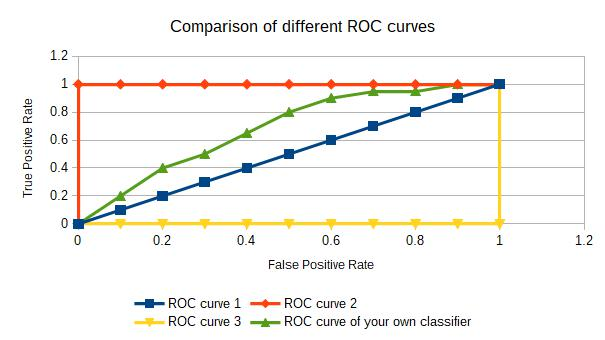
\includegraphics[scale=0.5]{ROC}\caption{\label{f.3.1}Comparison among different ROC curves}

\end{figure}

\begin{definition}AUC (area under curve) is a metric to measure the
``distance'' between the ROC curve generated by a classifier and
the extreme ROC curve 1. AUC is the area under the ROC curve generated
by a classifier and above the x-axis. 

\end{definition}

Note that $AUC$ is bounded between $0$ and $1$. If $AUC$ is close
to $0.5$, then ROC curve is close to the extreme ROC curve 1 and
we can conclude that the classifier is a poor classifier. If $AUC$
is close to $1\left(0\right)$, then the ROC curve is close to the
extrem ROC curve $2\left(3\right)$. The classifier in both cases
are consider good classifiers. (See Table \ref{t.3.1})

\begin{table}
\begin{tabular}{|c|c|c|}
\hline 
AUC & ROC curve of a classifier & Prediction\tabularnewline
\hline 
\hline 
close to 1 & close to the extreme ROC curve 2 & Very accurate\tabularnewline
\hline 
close to 1 & close to the extreme ROC curve 1 & no conclusions can be drawn\tabularnewline
\hline 
close to 0 & close to the extreme ROC curve 3 & Very inaccurate\tabularnewline
\hline 
\end{tabular}\caption{\label{t.3.1}Table to judge the quality of the classifier based on
AUC}

\end{table}

\end{document}
